\documentclass[a4wide,10pt]{article}
\usepackage{a4wide}
\usepackage[applemac,utf8]{inputenc}
\usepackage[danish]{babel}
\usepackage[T1]{fontenc}
\usepackage{pdfsync}
\usepackage{amsmath,amssymb,amsfonts} 
\usepackage[pdftex]{graphicx}
\usepackage{wrapfig}
\usepackage{color}
\usepackage[small,bf]{caption}

\begin{document}
\title{DSB Portfolio 1}
\author{Nis Sarup}
\date{\today}
\maketitle

\section{Draw the double sided spectrum of the amplitudes for the signal x(t)} % (fold)
\label{sec:draw_the_double_sided_spectrum_of_the_amplitudes_for_the_signal_x_t_}
By using Eulers princible $x(t)$ can be rewritten as:
\begin{eqnarray}
	x(t)&=&2\cdot \frac{e^{i2\pi \cdot 1000t}+e^{i2\pi \cdot 1000t}}{2}+\frac{e^{i2\pi \cdot 3000t}+e^{i2\pi \cdot 3000t}}{2}+\frac{e^{i2\pi \cdot 19000t}+e^{i2\pi \cdot 19000t}}{2} \nonumber \\
	x(t)&=&e^{i2\pi \cdot 1000t}+e^{i2\pi \cdot 1000t}+\frac{1}{2} \cdot e^{i2\pi \cdot 3000t}+\frac{1}{2} \cdot e^{-i2\pi \cdot 3000t}+\frac{1}{2} \cdot e^{i2\pi \cdot 19000t}+\frac{1}{2} \cdot e^{-i2\pi \cdot 19000t}
\end{eqnarray}
Which gives us the coefficients:
\begin{eqnarray}
	c_1&=&1 \nonumber \\
	c_{-1}&=&1 \nonumber \\
	c_3&=&0,5 \nonumber \\
	c_{-3}&=&0,5 \nonumber \\
	c_{19}&=&0,5 \nonumber \\
	c_{-19}&=&0,5 \nonumber \\
\end{eqnarray}
And the double sided spectrum:
\begin{figure}[htbp]
	\centering
		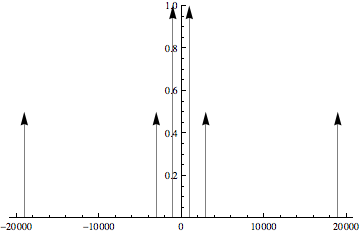
\includegraphics[width=8cm]{images/double-sided-spectrum-1.png}
	\caption{Double Sided Spectrum without aliasing}
	\label{fig:images_double-sided-spectrum-1}
\end{figure}

% section draw_the_double_sided_spectrum_of_the_amplitudes_for_the_signal_x_t_ (end)

\newpage

\section{Draw the double sided spectrum xs1(t) for the sampled signal without the
anti-aliasing filter} % (fold)
\label{sec:draw_the_double_sided_spectrum_xs1_t_for_the_sampled_signal_without_the_anti_aliasing_filter}
The samplerate of the A/D-converter is 20kHz. The new coefficients will be calculated by by multiplying them with the samplerate. Which gives:
\begin{eqnarray}
	c_1&=&20000 \nonumber \\
	c_{-1}&=&20000 \nonumber \\
	c_3&=&10000 \nonumber \\
	c_{-3}&=&10000 \nonumber \\
	c_{19}&=&10000 \nonumber \\
	c_{-19}&=&10000 \nonumber \\
\end{eqnarray}
And a plot of the double sided spectrum:
\begin{figure}[htbp]
	\centering
		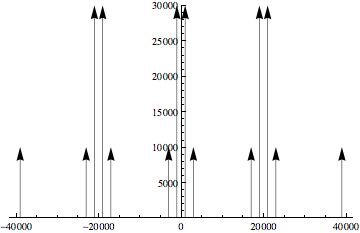
\includegraphics[width=8cm]{images/double-sided-spectrum-2.png}
	\caption{Double Sided Spectrum with aliasing}
	\label{fig:images_double-sided-spectrum-2}
\end{figure}
% section draw_the_double_sided_spectrum_xs1_t_for_the_sampled_signal_without_the_anti_aliasing_filter (end)
\newpage

\section{Calculate the A/D converter signal in dB} % (fold)
\label{sec:calculate_the_a_d_converter_signal_in_db}
A/D-converter signal can be calculated by using:
\begin{equation}
	SNR_{dB} = 10,79 + 20 \cdot Log_{10}(\frac{x_{rms}}{\Delta})
\end{equation}
Where:
\begin{equation}
	\Delta = \frac{x_{max} - x_{min}}{2^m}
\end{equation}
$x_{max}$ and $x_{min}$ is the maximum and minimum voltage for the A/D-converter and $m$ is the bitsize.
$x_{rms}$ is given by:
\begin{equation}
	x_{rms} = \sqrt{\frac{1}{T}\int_0^T x(t)^2 dT}
\end{equation}
We can then start calcualting:
\begin{eqnarray}
	x_{rms} &=& \sqrt{3} \nonumber \\
	\Delta = \frac{2 - (-2)}{2^8} &=& \frac{1}{64} \nonumber \\
	SNR_{dB} = 10,79 + 20 \cdot Log_{10}(\frac{\sqrt{3}}{\frac{1}{64}}) &=& 51,6848dB \nonumber
\end{eqnarray}
$SNR_{dB}$ is the strength of the signal.
% section calculate_the_a_d_converter_signal_in_db (end)

\section{Determine the quantization voltage for the A/D converter} % (fold)
\label{sec:determine_the_quantization_voltage_for_the_a_d_converter}
Quantization is the steps in which the A/D-converter moves. It is the same as $\Delta$ which we calculated in the previous section:
\begin{equation}
	\Delta = \frac{2 - (-2)}{2^8} = \frac{1}{64} \nonumber \\
\end{equation}
% section determine_the_quantization_voltage_for_the_a_d_converter (end)

\section{Determine the order of the filter for the analog Butterworth} % (fold)
\label{sec:determine_the_order_of_the_filter_for_the_analog_butterworth}
The equation can be converted to dB and solved with regards to n:
\begin{eqnarray}
	-48dB &=& 20 \cdot log_{10}(\frac{1}{\sqrt{1+(\frac{10000}{3000})^{2n}}}) \nonumber \\
	n = 4,58997 &\sim& 5 \nonumber
\end{eqnarray}
The order of the filter is 5.
% section determine_the_order_of_the_filter_for_the_analog_butterworth (end)
\newpage

\section{Determine the damping of the amplitude of the analog signal with 1000, 3000
or 10000 Hz} % (fold)
\label{sec:determine_the_damping_of_the_amplitude_of_the_analog_signal_with_1000_3000_or_10000_hz}
\begin{eqnarray}
	20 \cdot Log_{10}(\frac{1}{\sqrt{1+(\frac{1000}{3000})^{2\cdot 5}}}) &=& -0,00074dB \nonumber \\
	20 \cdot Log_{10}(\frac{1}{\sqrt{1+(\frac{3000}{3000})^{2\cdot 5}}}) &=& -3,0103dB \nonumber \\
	20 \cdot Log_{10}(\frac{1}{\sqrt{1+(\frac{10000}{3000})^{2\cdot 5}}}) &=& -52,2879dB \nonumber \\
\end{eqnarray}
% section determine_the_damping_of_the_amplitude_of_the_analog_signal_with_1000_3000_or_10000_hz (end)
\newpage

\section{Draw the double-sided spectrum xs2 for the sampled signal with the designed anti-aliasing filter} % (fold)
\label{sec:draw_the_double_sided_spectrum_xs2_for_the_sampled_signal_with_the_designed_anti_aliasing_filter}
Calculating magnitudes for frequencies 1000Hz, 3000Hz and 1900Hz:
\begin{eqnarray}
	\frac{1}{\sqrt{1+(\frac{1000}{3000})^{2\cdot 5}}} &=& 0,999992 \nonumber \\
	\frac{1}{\sqrt{1+(\frac{3000}{3000})^{2\cdot 5}}} &=& 0,707107 \nonumber \\
	\frac{1}{\sqrt{1+(\frac{19000}{3000})^{2\cdot 5}}} &=& 0,000098 \nonumber \\
\end{eqnarray}
These magnitudes are multiplied by the coefficients and the 10kHz sample frequency to get the real magnitudes:
\begin{eqnarray}
	0,999992 \cdot 1 \cdot 10kHz &=& 9999,92 \nonumber \\
	0,707107 \cdot 0,5 \cdot 10kHz &=& 3535,54 \nonumber \\
	0,000098 \cdot 0,5 \cdot 10kHz &=& 0,49 \nonumber \\
\end{eqnarray}
Double sided spectrum plot. The third signal is left out as it is so small compared to the two others:
\begin{figure}[htbp]
	\centering
		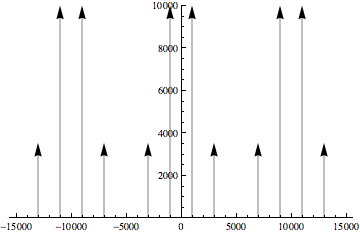
\includegraphics[width=8cm]{images/double-sided-spectrum-3.png}
	\caption{Double Sided Spectrum}
	\label{fig:images_double-sided-spectrum-3}
\end{figure}
% section draw_the_double_sided_spectrum_xs2_for_the_sampled_signal_with_the_designed_anti_aliasing_filter (end)
\newpage

\section{Calculate the filter order n for an reconstruction filter of Butterworth type} % (fold)
\label{sec:calculate_the_filter_order_n_for_an_reconstruction_filter_of_butterworth_type}
By adapting and making two equations we can solve two variables:
\begin{eqnarray}
	-0,5dB &\leq& 20 \cdot Log_{10}(\frac{1}{\sqrt{1+(\frac{3000}{f_c})^{2n}}}) \nonumber \\
	20 \cdot Log_{10}(\frac{1}{\sqrt{1+(\frac{10000}{f_c})^{2n}}}) &=& 20 \cdot Log_{10}(\frac{1}{\sqrt{1+(\frac{3000}{f_c})^{2n}}}) \nonumber \\ \nonumber
	n = 5,5 &\sim& 6 \nonumber \\
	f_c &=& 3636,87 \nonumber \\
\end{eqnarray}
The order of the filter is 6.
We then find the limits of $f_c$:
\begin{eqnarray}
	-48dB &\leq& 20 \cdot Log_{10}(\frac{1}{\sqrt{1+(\frac{10000}{f_c})^{2 \cdot 6}}}) \nonumber \\
	f_c &\leq& 3981,08 \nonumber \\
	-0,5dB &\geq& 20 \cdot Log_{10}(\frac{1}{\sqrt{1+(\frac{3000}{f_c})^{2 \cdot 6}}}) \nonumber \\
	f_c &\geq& 3574,81 \nonumber \\
\end{eqnarray}
$f_c$ must lie between 3574,81 and 3981,08. $f_c$ is set to 3700.
And the new filter:
\begin{equation}
	20 \cdot Log_{10}(\frac{1}{\sqrt{1+(\frac{3000}{3700})^{2 \cdot 6}}})
\end{equation}
% section calculate_the_filter_order_n_for_an_reconstruction_filter_of_butterworth_type (end)
\end{document}